% Chapter Template

\chapter{System Implementation} % Main chapter title

\label{Chapter5} % Change X to a consecutive number; for referencing this chapter elsewhere, use \ref{ChapterX}

\lhead{Chapter 5. \emph{System Implementation}} % Change X to a consecutive number; this is for the header on each page - perhaps a shortened title
The software framework proposed and introduced in \ref{Chapter4} has been exploited to develop the experimental platform. In this chapter the software architecture of the experimental platform is presented. Apart from the architecture itself, specific implementation details of each of the components in the system is also described in this chapter.  The software is designed using a hierarchical structure. The main layers of the system are
\begin{itemize}
\item \emph{Hardware Layer} is composed of sensors and robots connected to the network. Currently only those sensors that support TCP/IP network communication are considered.
\item \emph{Distributed Components Layer} is composed of individual processes that could be running across different computers/devices in the network
\item \emph{Application Components Layer} is the central server of the experimental platform which contains the backend processing units for the application to run as a whole.
\item \emph{User Interface Layer} takes the responsibility of providing useful and intuitive user-interface to the end users.
\end{itemize}
The architecture of the system shown in Fig~\ref{fig:architecture}. More finer details of each of the layers are presented in the following Sections~\ref{ssec:app_comp}$\sim$\ref{ssec:ui_comp}.

\begin{figure}
\centering
\begin{subfigure}[t]{0.48\textwidth}
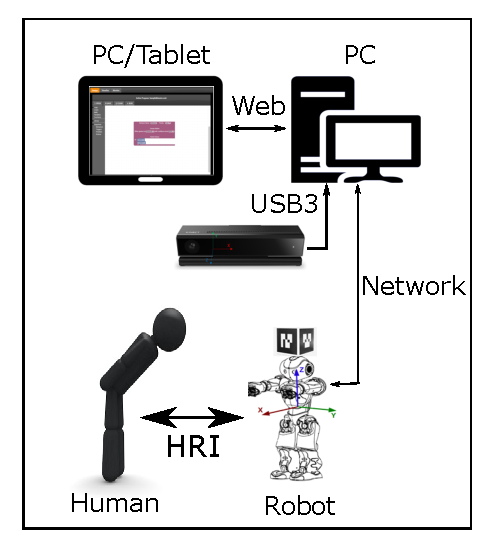
\includegraphics[width=\textwidth]{../thesis/assets/system_setup.eps}
\caption[System setup]{System setup}
\label{fig:localize_frames}
\end{subfigure}
\begin{subfigure}[t]{0.48\textwidth}
\includegraphics[width=\textwidth]{../thesis/assets/architecture.eps}
\caption[Software architecture]{Software architecture}
\label{fig:architecture}
\end{subfigure}
\caption[Experimental platform]{Experimental platform}
\label{fig:nao_localization}
\end{figure}
% \begin{figure}
% \centering
% \includegraphics[width=0.7\textwidth]{assets/architecture.eps}
% \caption[System Architecture]{System Architecture}
% \label{fig:architecture}
% \end{figure}
\section{Application Components}
\label{ssec:app_comp}
The application level components are responsible for bootstrapping and maintain the uptodate status of the system. 
\subsection*{Context}
The application context contains the complete description of the world. It contains latest information about
\begin{itemize}
\item Robot(s): A list of robots in the environment along with their 6D pose, Sensor information like Joint values etc.,
\item Human(s): A list of humans with their Skeleton Positions and Orientation, Active Gestures/Motions
\item Object(s): A list of manipulable objects in the environment along with their properties like description, color etc.,
\item Gesture Modules : A set of gesture recognition modules registered in the system that can actively provide information about the gestures of the humans in the environment.
\item Robot Behavior Modules: A set of robot behavior execution modules registered in the system.
\end{itemize}
The data structure of the context is shown in Fig~\ref{fig:system_context}
\begin{figure}
\centering
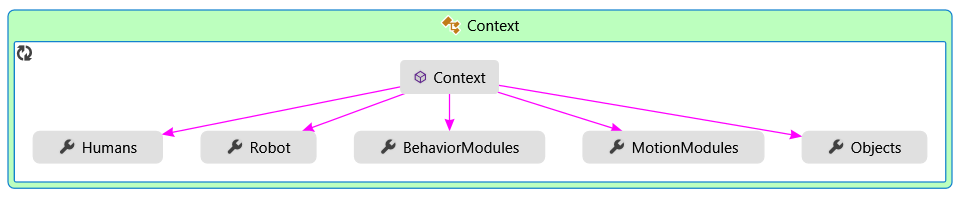
\includegraphics[width=\textwidth]{assets/context_diagram.png}
\caption[Application Context]{Application Context}
\label{fig:system_context}
\end{figure}
\subsection*{Parameter Server} 
The parameter server acts as a central repository for managing the parameters of the system and of the distributed components. The parameter server is basically designed as a responder socket which responds to the requests from a remote client. The list of supported request to pull the data from the parameter server is shown in the Table~\ref{table:parameter_server}
\begin{table}[H]
\centering
\small
\caption{Parameter Server Interface Specification}
\label{table:parameter_server}
\begin{tabular}{| p{3.3cm} | p{7.4cm} | p{2.8cm} |}
\hline
  \textbf{Request Description} & \textbf{Request Arguments} & \textbf{Response}
  \tabularnewline \hline
  Node Parameters request & \begin{itemize}[leftmargin=*,topsep={0pt},itemsep={0pt},partopsep={0pt},parsep={0pt}] 
                                                  \item Name of the node: string
                                                  \end{itemize} & Node Parameters 
                                          \tabularnewline\hline
                                          
  Motion recognition module registration request &  \begin{itemize}[leftmargin=*,topsep={0pt},itemsep={0pt},partopsep={0pt},parsep={0pt}] 
                                                  \item Name of the node: string
                                                  \item Module Information: GestureRecognitionModule
                                                \end{itemize} & Registration Status  (Success/Failure)
                                          \tabularnewline\hline
  
  Robot Interface module registration request & \begin{itemize}[leftmargin=*,topsep={0pt},itemsep={0pt},partopsep={0pt},parsep={0pt}] 
                                                \item Name of the node: string
                                                \item Module Information: RobotBehaviorModule 
                                            \end{itemize} & Registration Status  (Success/Failure)
                                          \tabularnewline\hline
  File Request & \begin{itemize}[leftmargin=*,topsep={0pt},itemsep={0pt},partopsep={0pt},parsep={0pt}] 
                                                  \item Name of the file
                                                  \end{itemize} & Contents of the File  
  										 \tabularnewline\hline
\end{tabular}
\end{table}
\subsection*{Context Orchestrator} The orchestrator collect uptodate information about the robots and humans in the environment from the perception system and updates the Context. The algorithm used by the orchestrator to update the context information is shown below.

\begin{algorithm}[H]
 \KwData{(app\_config, context)}
 \textbf{\emph{Init}}:\\
 \quad PUBLISHERS = READ\_ALL\_PUBLISHER\_INFO(app\_config)\;
 \quad SUBSCRIBERS = CREATE\_SUBSCRIBERS(PUBLISHERS)\;
 \While{run}{
 	\ForAll{SUBSCRIBER in SUBSCRIBERS}{ 
 		data = RECEIVE\_DATA(SUBSCRIBER,TIME\_OUT)\;
 		UPDATE\_CONTEXT(context, data)\;
 	}
 }
 \caption{Context Synchronization Algorithm}
 \label{alg:context_sync}
\end{algorithm}
\subsection*{Embedded Web server}
The web server embedded in the application serves the file and data requests from the web client. The server side server implements a set of RESTful services which could be accessed from the web clients. The JSON data format which is the default standard for modern web interface development has been used as data exchange format between the server and the web clients. The list of RESTful API implemented on the server side is shown in Table~\ref{table:restful_api}
\begin{table}[H]
\centering
\small
\caption{Embedded Web Server RESTful API}
\label{table:restful_api}
\begin{tabular}{|l|p{2.8cm}|p{1.2cm}|p{5.5cm}|}
\hline
  \textbf{Request Url}  & \textbf{Parameters} & \textbf{Request Type} & \textbf{Description/Response}
  \tabularnewline \hline
  /models/{type}/(?$<$all$>$.*) & File Name & GET & Robot 3D Model Data
                                          \tabularnewline\hline
                                          
  /context  & - & GET & Current context data  
  										                    \tabularnewline\hline
  										 
  /robot  &  - & GET & Default Robot information  
  										                    \tabularnewline\hline										 
  
  /humans & - & GET  & Information about all the human in the environment  
                                          \tabularnewline\hline
                                          
  /human/\{id\} & id - Human Id & GET  & Information about the human with the given id.  
                                          \tabularnewline\hline
                                          
  /jointvals & - & GET  & Joint values of the default robot  
                                          \tabularnewline\hline
                                          
  /visualize/skeleton/list & - & GET  & 3D Skeleton positions of all the humans in the environment  
                                          \tabularnewline\hline                                        
       
  /designer/program/list & - & GET  & List of all the behavior programs stored in the server  
                                          \tabularnewline\hline                                                               
                                          
  /designer/program/start & Behavior Program & POST  & Request the bootstrapper to start the program
  										                    \tabularnewline\hline   

  /designer/program/save & File Name, Behavior Program & POST  & Request the bootstrapper to start the program
                                          \tabularnewline\hline 
  /designer/program/stop & - & POST  & Request to stop running program if any
                                          \tabularnewline\hline
\end{tabular}
\end{table}

\subsection*{Bootstrapper} 
The bootstrapper takes care of initializing the system and starting up all the pre-configured nodes. The configuration information of the nodes is specified using the XML configuration file described in Section~\ref{sec:config_file}. It also takes of starting and stopping the behavior programs when requested by the user. The sequence operations of bootstrapper performs is represented in Algorithm~\ref{alg:bootstrapper}.

\begin{algorithm}[H]
 \KwData{(XML Config File)}
 \textbf{\emph{Startup}}:\\
 \quad INIT\_AND\_RUN\_PARAMETERSERVER()\;
 \quad INIT\_AND\_RUN\_CONTEXTSYNC()\;
 \quad INIT\_AND\_RUN\_CONTEXTSERVER()\;
 \quad INIT\_AND\_RUN\_WEBSERVER()\;
 \quad NODES = GET\_NODES(XML Config File)\;
 \quad PROCESSES = []\;
 \ForAll{NODE in NODES}{ 
 	\If{NODE is ENABLED}{
 		PROCESS = CREATE\_PROCESS(NODE)\;
 		APPEND(PROCESSES, PROCESS)
 	} 
 }
 \While{run}{
 	MONITOR(PROCESSES)
 }
 \textbf{\emph{Shutdown}}:\\
 \quad SHUTDOWN\_WEBSERVER()\; 
 \quad SHUTDOWN\_CONTEXTSERVER()\;
 \quad SHUTDOWN\_CONTEXTSYNC()\;
 \quad SHUTDOWN\_PARAMETERSERVER()\;
 \quad SHUTDOWN(PROCESSES)
 \caption{Bootstrapper Algorithm}
 \label{alg:bootstrapper}
\end{algorithm}
\section{Distributed Components}
\label{ssec:dist_comp}
These are nodes in the system each with a specific goal that can be started/stopped at any time during the entire application life-cycle without affecting the other nodes or the system. All the nodes will communicate with the application using message passing techniques. They can run in any machine inside the network.

\subsection{Motion Recognition Node} A dedicated node that interacts with a motion recognition sensor and sends the detected gestures and motions to the application. Additionally each motion recognition module registers a set of actions/gestures that could be detected with the sensor associated with it. The gesture recognition logic depends on the sensor associated with the gesture recognition module. The gesture recognition workflow of kinect based system in explained in Section~\ref{sssec:kinect_gestures}
\subsubsection{Kinect Gesture Recognition}
\label{sssec:kinect_gestures}
	The Microsoft Kinect system utilizes Adaptive Boosting(adaboost) algorithm \cite{freund1997decision} to efficiently detect the gestures. The system involves a training phase during which the desired gestures are captured and tagged. These tagged gestures will be used by a gesture detector trainer which will generate a set of training examples. The training results are stored in files and will be used by the gesture detector to perform per-frame classification of the data. The Visual Gesture Builder (VGB) tool that comes together with Kinect for Windows SDK eases the process of tagging the gestures, evaluating the gesture recognition and creating the gesture database. The work-flow of using the VGB is shown in the Figure~\ref{fig:vgb_workflow}.
\begin{figure}[H]
\centering
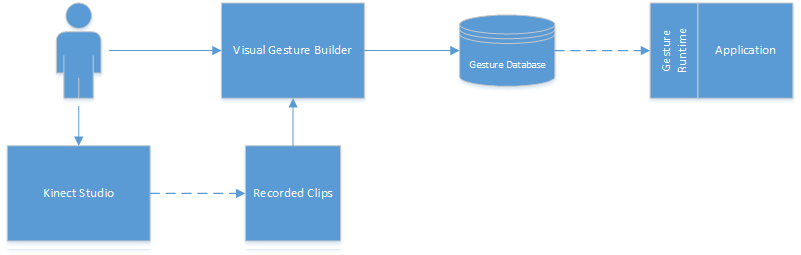
\includegraphics[width=0.8\textwidth]{assets/VisualGestureBuilder.png}
\caption[Visual Gesture Builder Work flow]{Visual Gesture Builder Work flow \cite{KinectSDK2014}}
\label{fig:vgb_workflow}
\end{figure}
% Motion recognition
The workflow shown in Figure~\ref{fig:vgb_workflow} has been adopted to develop all the gestures needed for the kinect gesture recognition module. The process followed for generating the Left hand wave gesture is shown in the Figure~\ref{fig:gesture_waveleft}. As shown in the figure at first the clips are captured using the Kinect studio tool and  stored as \textbf{XEF} files. The clips are then imported in the visual gesture builder. The imported clips could be traversed and the tagging is done (i.e at each frame it is possible to specify if that particular frame is part of the gesture of interest or not). This process could be repeated on one or more imported clips. The tagged clips are built in order to generate a set of weak classifiers and learn confidence values for each of those classifiers. Once the training process is complete, the trained classifier could be evaluated over a set of test clips using a live preview as shown in step 3 in the figure. When the results are satisfactory, the training data could be exported as a database saved as \textbf{VGD} (Visual Gesture Database) format.
\begin{figure}[H]
\centering
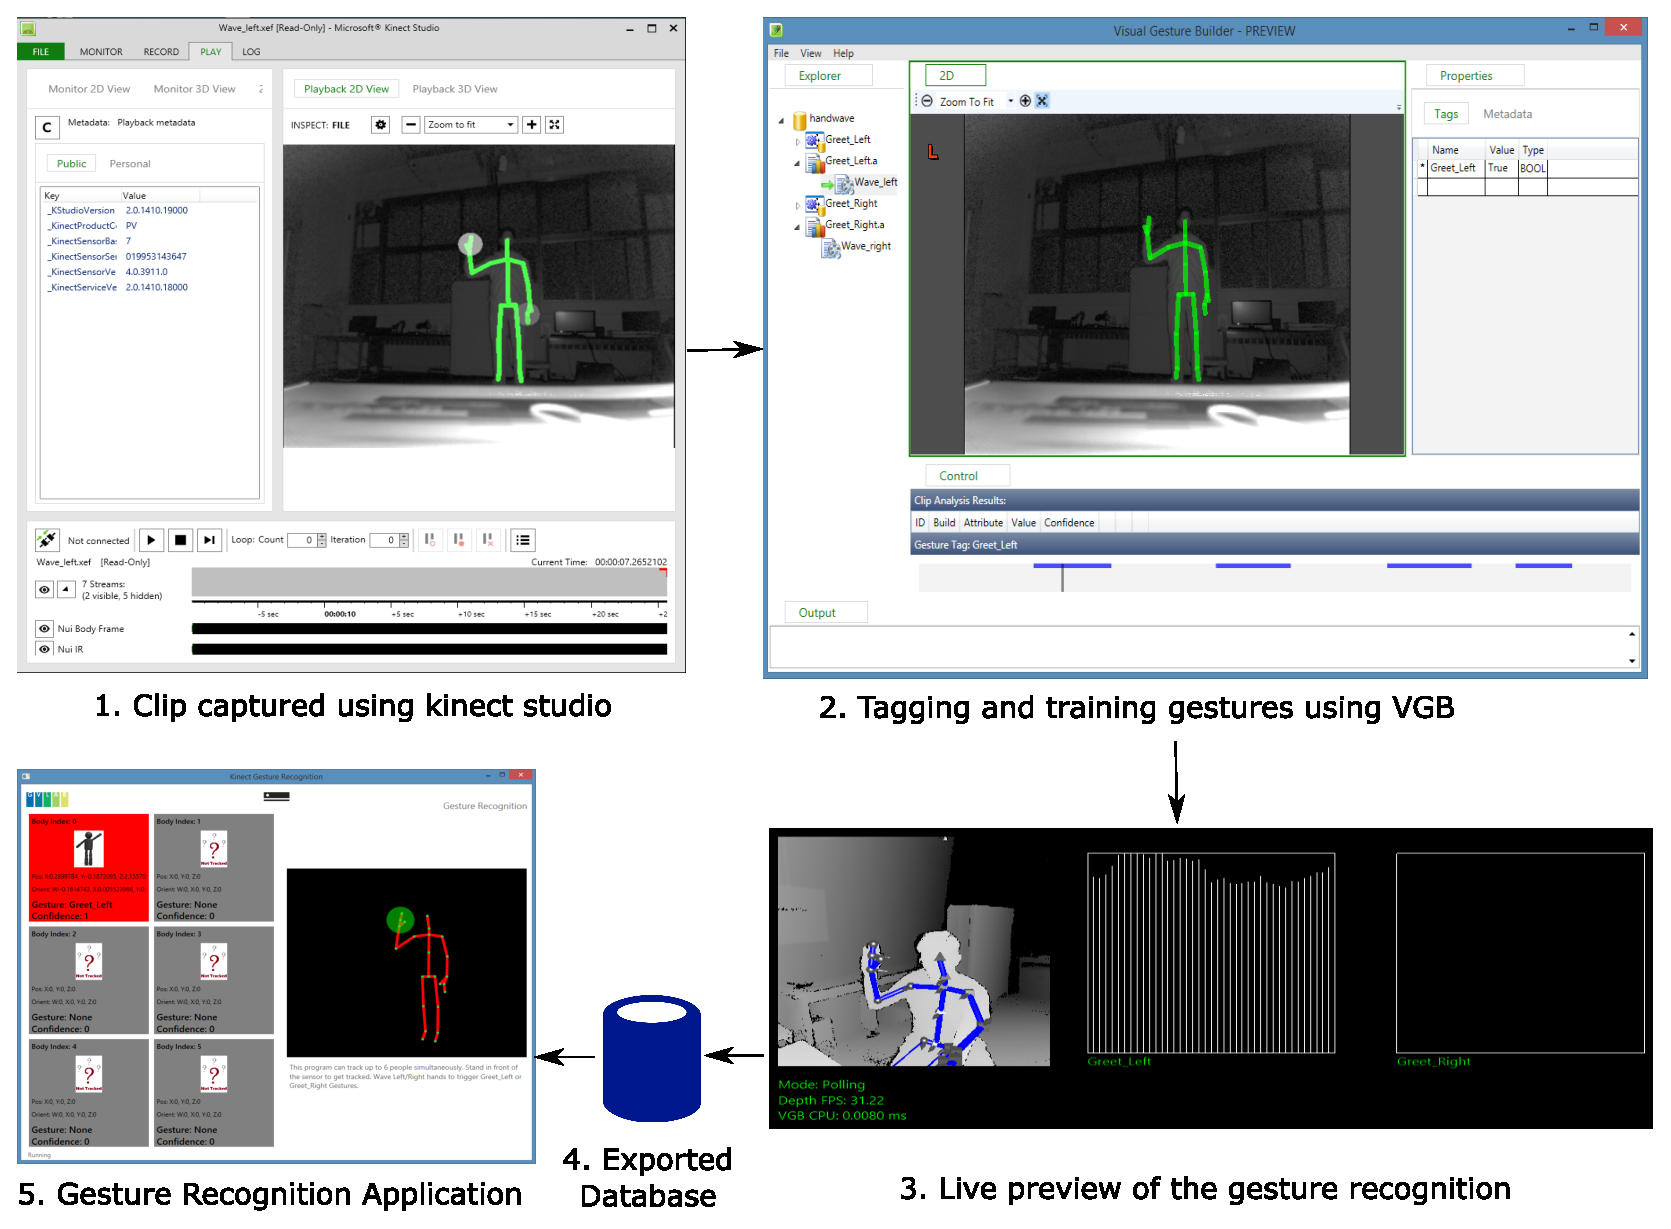
\includegraphics[width=\textwidth]{assets/gesture_recog_flow.eps}
\caption[Left hand wave gesture work flow]{Left hand wave gesture work flow}
\label{fig:gesture_waveleft}
\end{figure}
The database is imported into the gesture recognition module and the responsibility of this module is to notify any interested subscribers when a gesture is recognized. Additionally this module also publishes information about the skeletons of the humans in view. The algorithm of this module is shown in Algorithm~\ref{alg:gesture_recognize}

\begin{algorithm}[H]
 \KwData{Gesture database}
 \KwResult{Gesture Triggers}
 \textbf{\emph{Init}}:\\
 \quad gestures = READ\_DATABASE()\;
 \quad REGISTER\_GESTURES(gestures)\;
 \While{True}{
  skeletons = GET\_SKELETONS()\;
  \ForAll{gesture in gestures}{ 
    detected = DETECT\_GESTURE(gesture)\;
    \If{detected}{
      PUBLISH(gesture)\;
    } 
  }
  PUBLISH(skeletons)\;
 }
 \caption{Kinect Gesture Recognition Module}
 \label{alg:gesture_recognize}
\end{algorithm}
\subsection{Robot interface node} 
The Robot interface node is a dedicated node that interacts with a specific robot and can invoke a set of actions on it.  It registers a set of actions that could be invoked on the robot associated with it. The robot interface node sets up a publisher that periodically sends the information about the robot status like joint values, sensor information to the application to keep the context uptodate. Additionally it sets up a responder socket which will wait for action execution request from the remote node. The robot interface node dedicated to Nao humanoid robot is described in Section~\ref{sssec:nao_interface}
\subsubsection{NAO Robot Interface}
\label{sssec:nao_interface}
The Nao robot interface makes use of the NaoQi python SDK which provides API for accessing various functionalities of the robot such as joint/cartesian control, memory access, motion, speech, object/face/people detection and tracking, behavior invocation etc., A set of necessary functions are implemented in the NaoBehaviorModule and they are registered to the application when the node is started up. The control flow is shown in Figure~\ref{fig:nao_interface}.

\begin{figure}[H]
\centering
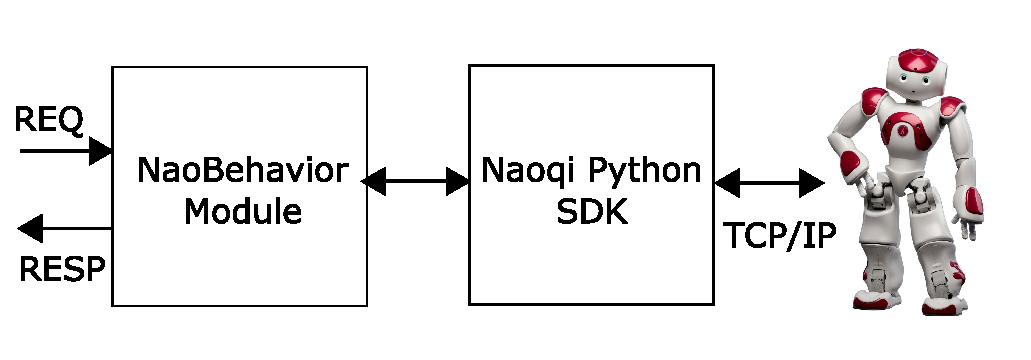
\includegraphics[width=0.7\textwidth]{assets/NaoBehaviorModule.eps}
\caption[NAO Robot Interface]{NAO Robot Interface}
\label{fig:nao_interface}
\end{figure}

\subsection{Localization Node} A dedicated node which uses the perception system to resolve and publish the current position of the robot.

\subsubsection{NAO Robot localization}
The fiducial marker based approach is used in order to localize the robot in the field of view of the Kinect sensor. The ALVAR \cite{ALVAR} toolkit is used for marker detection purpose which relies on OpenCV library for image processing. The OpenCV library cannot directly read the image streams from Kinect sensor and hence a OpenCV compatible driver is implemented to read the RGB image streams. The first step in the marker detection is to calibrate the camera in order to get its intrinsic parameters and the calibration parameters are stored in an XML file. A set of supported markers of known identifiers are chosen and a cube of known geometry is created. The cube is designed in such a way that at any instant atleast one of the markers will be detected if the robot is in the detectable range of the camera. The cube is mounted on the head of NAO robot since it will avoid the problem of occlusion in most cases. However since the head of the NAO has 2 DOF which will result in the movement of mounted cube even if the robot itself does not move. In order to overcome this problem, a kinematic model of the NAO humanoid robot from torso frame to tip of the head frame parameterized using Modified Denavit Hartenberg (MDH) \cite{khalil2004modeling} parameters is used. The MDH parameters are shown in Table~\ref{table:nao_mdh}.

\begin{table}[H]
\centering
\small
\caption{MDH parameters from Torso to top of head}
\label{table:nao_mdh}
% \begin{tabular}{|l|l|p{1cm}|p{1cm}|p{1cm}|p{1cm}|p{3cm}|}
\begin{tabular}{|l|l|c|c|c|c|p{2cm}|}
\hline
  \textbf{$i$}  & \textbf{$j$}  & \textbf{$\alpha_j$ (rad)} & \textbf{$d_j$ (mm)} & \textbf{$\theta_j$ (rad)} & \textbf{$r_j$ (mm)} & \textbf{Description}
  \tabularnewline \hline
  - & 0 & 0 & 0 & 0 & 0 & Torso/Base
                                          \tabularnewline\hline
                                          
  0 & 1 & 0 & 0 & $\theta_1$ & 126.50 & Head Yaw
                                          \tabularnewline\hline
                       
  1 & 2 & $-\frac{\pi}{2}$ & 0 & $\theta_2$ & 0 & Head Pitch
                                          \tabularnewline\hline                    
  
  2 & 3 & $\frac{\pi}{2}$ & 0 & 0 & 110.00 & Head Tip
                                          \tabularnewline\hline
\end{tabular}
\end{table}

\begin{figure}
\centering
\begin{subfigure}[t]{0.48\textwidth}
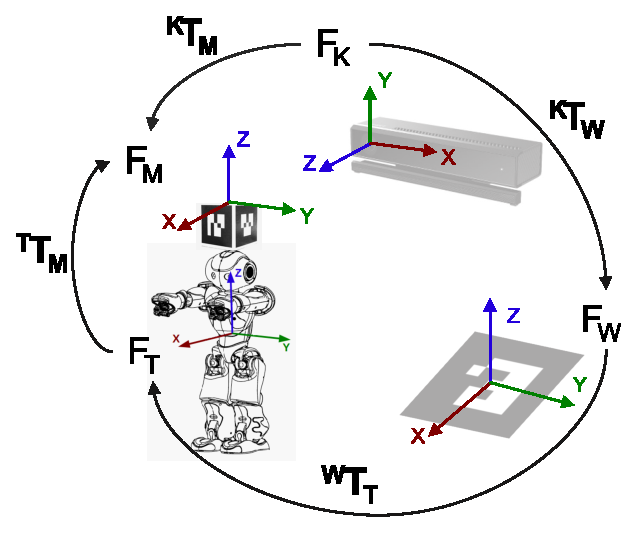
\includegraphics[width=\textwidth]{../thesis/assets/localization_concept2.eps}
\caption[Modeling]{Coordinate Frames}
\label{fig:localize_frames}
\end{subfigure}
\begin{subfigure}[t]{0.48\textwidth}
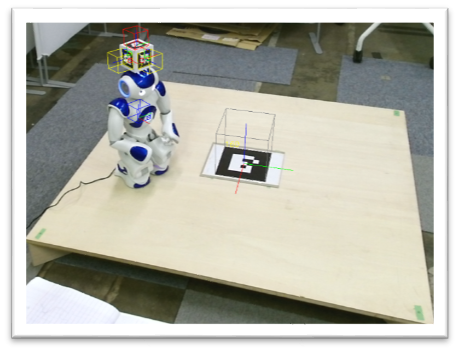
\includegraphics[width=\textwidth]{../thesis/assets/localization_frames.png}
\caption[Actual setup]{Actual setup}
\label{fig:localize_setup}
\end{subfigure}
\caption[NAO robot localization]{NAO robot localization}
\label{fig:nao_localization}
\end{figure}

\subparagraph{Modeling}
For computing the absolute pose of the torso frame of the robot with respect to the world frame, the coordinate frames shown in Figure~\ref{fig:nao_localization} is used. 

\begin{tabular}{r l}
\centering
  Kinect Frame & $F_K$ \\ 
  Marker Frame & $F_M$ \\ 
  Torso Frame & $F_T$ \\ 
  World Frame & $F_W$ \\ 
  Transformation Matrices  & ($^{K}T_M$,$^{T}T_M$,$^{K}T_W$,$^{W}T_T$) \\
\end{tabular}

The algorithm for the computation given the marker parameters, calibration information of the camera, MDH parameters (Table~\ref{table:nao_mdh}) and the joint values ($\theta_1,\theta_2$) at each time instant is shown in Algorithm~\ref{alg:localize}.

\begin{algorithm}
 \KwData{marker\_size, cube\_size, MDH\_Params}
 \KwResult{TORSO\_POSE}
 \textbf{\emph{Init}}:\\
 g\_model := INIT\_GEOM\_MODEL(MDH\_Params)\;
 m\_model := MARKER\_MODEL(marker\_size, cube\_size)\;
 \While{True}{
 	data = READ\_RGB\_STREAM()\;
  [$\theta_1$,$\theta_2$] = READ\_JOINT\_VALUES()\;
 	marker\_poses = DETECT\_CUBE\_MARKERS(data)\;
  $^{K}T_W$ = DETECT\_WORLD\_MARKER(data)\;
 	$^{K}{T}_{M}$ = TRANSFORM\_TO\_TOP\_FRAME(marker\_poses, m\_model)\;
 	$^{T}{T}_{M}$ = COMPUTE\_TOP\_FRAME(g\_model,$\theta_1$,$\theta_2$)\;
 	$^{K}{T}_{T}$ = $^{K}{T}_{M}$ $\times$ ${^{T}{T}_{M}}^{-1}$\;
  $^{W}{T}_{T}$ = ${^{K}{T}_{W}}^{-1}$ $\times$ ${^{K}{T}_{T}}$\;
 	TORSO\_POSE = MEDIAN\_FILTER($^{W}{T}_{T}$)\;
 	PUBLISH(TORSO\_POSE)\;
 }
 \caption{Localization Algorithm}
 \label{alg:localize}
\end{algorithm}

\section{Behavior Program} 
\label{ssec:behavior_program}
A dynamic component that will be created when the user starts the program he/she designed using the user interface. The declarative description of the behavior is parsed in order to create a memory model. The Behavior program node monitors the application context for the motion triggers and invokes the corresponding robot actions according to the way it is being described in the program.
\begin{figure}
\centering
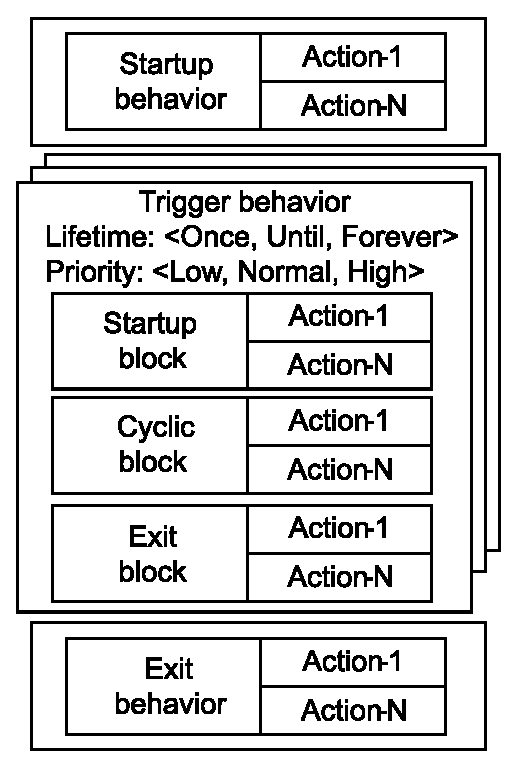
\includegraphics[width=0.4\textwidth]{../thesis/assets/program_structure.eps}
\caption[Behavior Program - Conceptual Model]{Behavior Program - Conceptual Model}
\label{fig:program_concept}
\end{figure}
\subsection{Conceptual Model}
The behavior program is structured in a simple way so that it could be easily understood by the end user. The conceptual model of behavior program is shown in Fig.~\ref{fig:program_concept}. The behavior program is composed of:
\begin{itemize}
\item \emph{Startup behavior}: The startup block will be executed once when the user starts the program. The user can add a set of actions to be performed when the program starts. The start-up block is optional and there cannot be more than one start-up block in the program
\item \emph{Trigger behavior}: The behavior block is the core component of the behavior program. The block could be activated by the interaction between the human and the robot. There could be many behavior blocks in a program. The properties/attributes of a behavior block is shown in Table~\ref{table:behavior_block}.
\begin{table}[H]
\centering
\small
\caption{Trigger Behavior block properties}
\label{table:behavior_block}
\begin{tabular}{|l|p{11cm}|}
\hline
  \textbf{Property} & \textbf{Description}
  \tabularnewline \hline
  
  Trigger & The signal that activates the behavior block. The trigger source could be either of human presence/absence, motion gesture, vicinity of human, verbal command or any boolean edge trigger.
                                          \tabularnewline\hline
                                          
  Lifetime & The lifespan of the behavior block. \begin{itemize}[leftmargin=*,topsep={0pt},itemsep={0pt},partopsep={0pt},parsep={0pt}]
                                                                      \item Once: The block will be executed only once.
                                                                      \item Forever: The block will be executed forever each time trigger condition is met.
                                                                      \item Until: The block will be executed until a condition is met
                                                                   \end{itemize}
                                          \tabularnewline\hline
  
  Priority & The priority of the block could be Low, Normal or High and the behavior execution is scheduled based on fixed-priority preemptive scheduling. There is not dynamic priority allocation as the concept could be confusing for naive users.
                                          \tabularnewline\hline

  Startup & Tasks/actions to be performed once when the block is initialized
                                          \tabularnewline\hline

  Cyclic & Tasks/actions to be performed each time the trigger condition is met
                                          \tabularnewline\hline
  
  Exit &  Tasks/actions to be performed once when the lifetime of the block expires
                                          \tabularnewline                                                                       
                      \hline
\end{tabular}
\end{table}
\item \emph{Exit behavior}: The exit block will be executed once when the lifetime of all the configured behavior blocks expire. Like the startup block there could be only one exit block in the program.
\end{itemize}
\subsection{Block level implementation}
The visual blocks corresponding to each of the startup, trigger and exit behaviors are implemented. The complex programs could be composed by putting together these blocks. The startup and exit blocks are shown in Fig~\ref{fig:blocks_init}. As could be seen from the figure, the blocks are quite simple making it possible to put the list of statements consisting of initialization and termination logic of the program. 
\begin{figure}[H]
\centering
\begin{subfigure}[t]{0.28\textwidth}
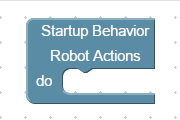
\includegraphics[width=\textwidth]{../thesis/assets/blocks_startup.png}
\caption[Startup block]{Startup block}
\label{fig:program_concept}
\end{subfigure}
\begin{subfigure}[t]{0.28\textwidth}
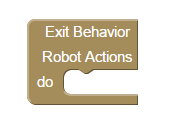
\includegraphics[width=\textwidth]{../thesis/assets/blocks_exit.png}
\caption[Exit block]{Exit block}
\label{fig:program_blocks}
\end{subfigure}
\caption[Startup and Exit behaviors]{Startup and Exit behaviors}
\label{fig:blocks_init}
\end{figure}
The trigger behavior block is designed in such a way that it incorporates the conceptual model and at the same time easier for the end user to understand and use it. The trigger behavior block is shown in Fig~\ref{fig:blocks_trigger}. The visual design provides ability to compose the blocks by putting an external boolean trigger, choose priority and lifetime from the combo box interface, add startup,cyclic and exit statements etc.,
\begin{figure}[H]
\centering
\begin{subfigure}[t]{0.38\textwidth}
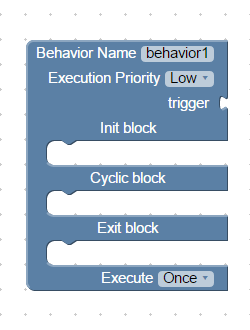
\includegraphics[width=\textwidth]{../thesis/assets/blocks_behavior1.png}
\caption[Example 1]{Priority: Low, Execute: Once}
\label{fig:program_concept}
\end{subfigure}
\begin{subfigure}[t]{0.38\textwidth}
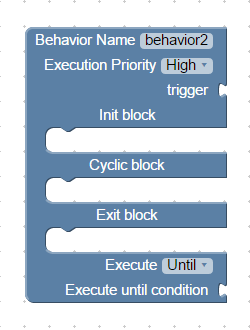
\includegraphics[width=\textwidth]{../thesis/assets/blocks_behavior2.png}
\caption[Example 2]{Priority: High, Execute: Until}
\label{fig:program_blocks}
\end{subfigure}
\caption[Trigger behavior]{Trigger behavior}
\label{fig:blocks_trigger}
\end{figure}
The block interface is reactive in the sense that for instance when the lifetime of the block is switched from \emph{Once/Forever} to \emph{Until}, a new input appears in the block where the user can add the condition to stop the block.
\subsection{Code Generation and Execution}

\section{User Interface}
\label{ssec:ui_comp}
The user interface is a web application that runs on any latest web-kit browsers supporting HTML5, CSS3 and WebGL technologies. The list of libraries and components used to build the web interface has been described in Section~\ref{sec:ui_design}. In this section the various screens in the developed user interface has been described. The UI is composed of tabbed interface consisting of 3 main components as shown in Fig~\ref{fig:behavior_designer}.
\begin{itemize}
\item Design: To design the behavior
\item Visualize: To visualize the interaction
\item Monitor: To visualize the human and robot information
\end{itemize}

\subsection{Behavior Designer} The Behavior designer surface could be used by the user to drag and drop the behavior blocks and construct the program using the set of motion capabilities registered by the active motion recognition nodes and the set of robot action capabilities registered by the active robot interface nodes. The behavior designer is shown in Fig~\ref{fig:behavior_designer}.

\begin{figure}[H]
\centering
\begin{tikzpicture}
    \node [anchor=north] (main) at (1.5,9.5) {\Large Main Tabs};
    \node [anchor=north] (cmd) at (5,9.5) {\Large Designer commands};
    \node [anchor=south] (toolbox) at (1.5,-1) {\Large Toolbox};
    \node [anchor=north] (name) at (10,9.5) {\Large Program name};
    \node [anchor=south] (surface) at (8,-1) {\Large Designer Surface};
    \node[anchor=south west,inner sep=0] (image) at (0,0) {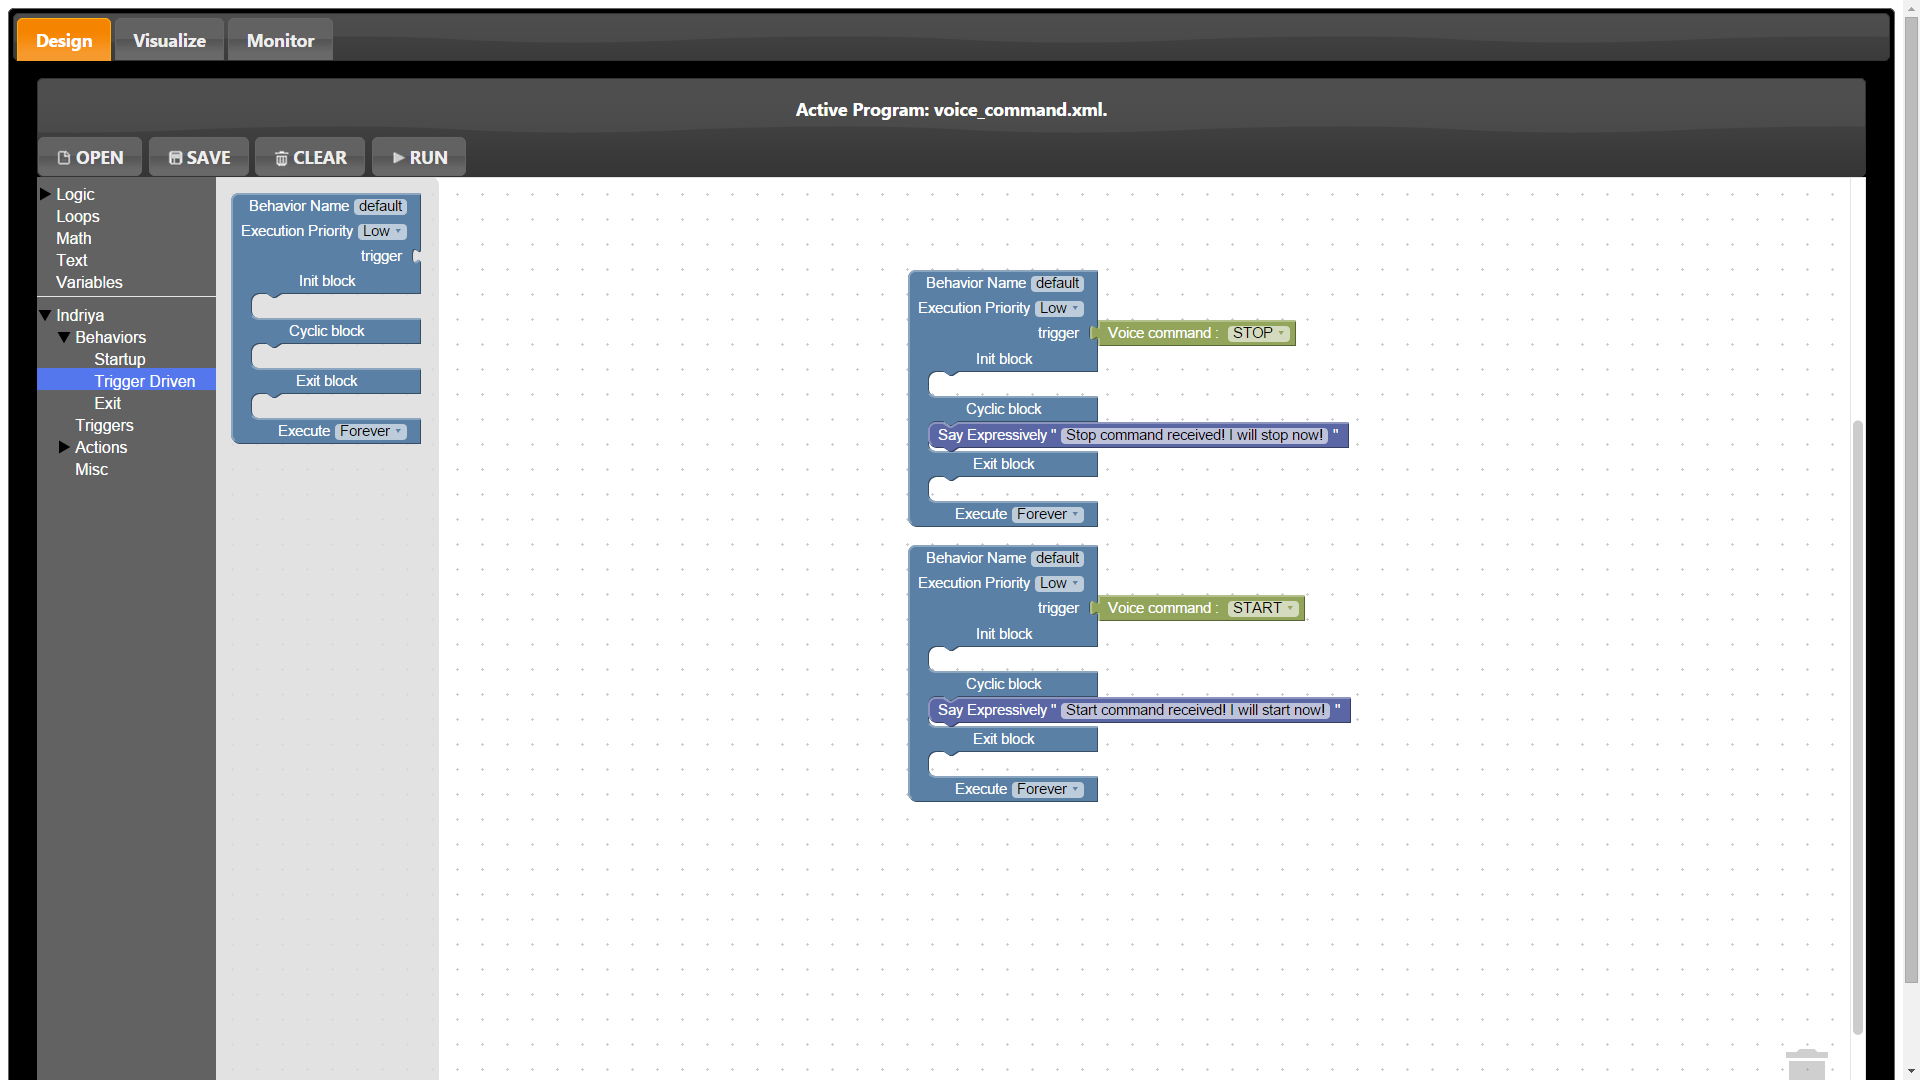
\includegraphics[width=\textwidth]{ui_designer.png}};
    \begin{scope}[x={(image.south east)},y={(image.north west)}]
        %\draw[red,ultra thick,rounded corners] (0.62,0.65) rectangle (0.78,0.75);
        \draw[red,ultra thick,rounded corners] (0,0.93) rectangle (0.22,0.99);
        \draw[red,ultra thick,rounded corners] (0,0.89) rectangle (0.25,0.84);
        \draw[green,ultra thick,rounded corners] (0,0.825) rectangle (0.23,0.01);
        \draw[yellow,ultra thick,rounded corners] (0.4,0.87) rectangle (0.6,0.93);
        \draw[blue,ultra thick,rounded corners] (0.235,0.825) rectangle (0.97,0.01);

        % \draw [-latex, ultra thick, red] (main) to[out=0, in=-120] (0.01,0.96);
        % \draw [-latex, ultra thick, red] (cmd) to[out=0, in=-120] (0.01,0.89);
        % \draw [-latex, ultra thick, green] (toolbox) to[out=0, in=-120] (0.05,0.5);
        % \draw [-latex, ultra thick, yellow] (name) to[out=0, in=-120] (0.5,0.87);
        % \draw [-latex, ultra thick, blue] (surface) to[out=0, in=-120] (0.5,0.5);
        \draw [-stealth, line width=3pt, red] (main) -- ++ (-0.0,-0.15);
        \draw [-stealth, line width=3pt, red] (cmd) -- ++ (-0.12,-0.24);
        \draw [-stealth, line width=3pt, green] (toolbox) -- ++ (0,0.5);
        \draw [-stealth, line width=3pt, yellow] (name) -- ++ (-0.1,-0.19);
        \draw [-stealth, line width=3pt, blue] (surface) -- ++ (0,0.5);
    \end{scope}
\end{tikzpicture}
    \caption[Behavior designer]{Behavior designer}
    \label{fig:behavior_designer}
\end{figure}

The behavior designer is the core component of the user interface. The designer is composed of 
\begin{itemize}
\item The command panel is composed of Designer command buttons like Open/Save/Clear/Run which makes it easy to perform operations like Creating a new program, Saving the program to the server, Clear the workspace and Running the active behavior program
\item The toolbox contains the collection of blocks categorized as per their functionlities.
\end{itemize}

\subsection{Visualization} The visualization could be used to see the interaction of the human and robot inside a virtual 3D environment.
% Simulation Node
\begin{algorithm}
 \KwData{simulation\_config}
 \textbf{\emph{Init}}:\\
 \quad INIT\_SIMULATION\_ENGINE(simulation\_config) \;
 \quad INIT\_SUBSCRIBERS(simulation\_config) \;
 \quad LOAD\_ENVIRONMENT(simulation\_config) \; 
 \While{True}{
 	sensors = READ\_SENSOR\_VALUES() \; 
 	skeletons = READ\_SKELETON\_DATA() \; 
 	RENDER(robot,sensors)
 }
 %\caption{Localization Algorithm}
 %\label{alg:localize}
\end{algorithm}

\subsection{Monitor}

\section{Summary}
